The widespread use of information-rich technologies in the life sciences has spurred a lively crosstalk with research in machine learning, with the goal of improving how we explore and derive conclusions from biological data. 

The most prevalent use of machine learning in this setting is \textit{supervised learning}, where one makes use of any available observations in order to make inferences about measurable, yet unobserved quantities of interest. Consider as an example the case of a clinical study where one is interested to predict the outcome (discrete or quantitative) of treatments based on input covariates of environmental, genetic or other molecular origin~\cite{Rajkomar2018, Dincer2018a}. In supervised learning, the input covariates (normally denoted by $x$) are usually available for all participants in the study, while the treatment outcome (i.e., the target, denoted by $y$) is only available for a subset of them. A classical approach to predict $y$ in those missing cases is to learn a conditional distribution $p\left(y \mid x \right)$ -- namely what is the probability for a certain outcome $y$ given any environmental or molecular information represented by $x$. Such an approach is referred to as \textit{discriminative learning} and includes methods such as random forests, support vector machines, linear models, and neural networks; We refer the reader to~\cite{Wainberg2018, Eraslan2019, Ching2018, Zou2019} for reviews on the use of neural networks for supervised learning in biological settings.


While discriminative learning is a powerful approach, our focus in this thesis is on \textit{generative} modeling -- an alternative approach which models explicitly the joint distribution $p\left(x, y\right)$. Naturally, generative modeling is attempting to solve a harder statistical problem, as it seeks to model the uncertainty in the input covariates $x$ as well. Even though discriminative approaches generally have superior performance in the prediction problem, generative models can sometimes be preferred as they can account for domain knowledge about how the data in $x$ were generated~\cite{ng2002discriminative}. For instance, if $x$ represents an amino acid sequence, then the probability that $x$ occurs in nature can be better estimated by a generative model that accounts for interactions between residues~\cite{Riesselman2018}. 


Explicitly modeling $x$ means that generative models can also be used to generate new instances of $x$ \textit{in-silico}. This capacity opens the way for additional applications that can aid with and even go beyond the prediction problem. Specifically, data generation can be used for identifying values of $x$ that were not previously observed but are likely to be associated with a desirable value of $y$. This was used, for instance, to propose new chemical compounds (represented by $x$) that are likely to have a certain melting temperature (represented by $y$)~\cite{Sanchez-Lengeling2017}. Addition of new, artificial data points to an available set of observations has also been useful for increasing the performance of classifiers, e.g., in the context of predicting drug effects with fluorescence microscopy~\cite{lafarge2018capturing}.   

The use of generative models also extends beyond supervised learning, i.e., for cases where one does not have a target output to predict. In this \textit{unsupervised} regime, we are interested in finding patterns in $x$, with common tasks including identifying measurements errors (outlier detection~\cite{Ding2018}), inferring the values of missing entries in $x$ (imputation~\cite{pmlr-v97-mattei19a}), or otherwise identifying latent sources of variation that give rise to the data (dimensionality reduction or embedding~\cite{Lopez2018}). Notably, it is important to note that the embeddings are commonly used for partitioning the data into groups (clustering). Generative modeling has emerged as a powerful paradigm to address these tasks due to its ability to directly model $x$. For instance, in single cell-RNA sequencing (where $x$ corresponds to gene expression values in each cell) a common practice is to model $x$ by conditioning on a small set of latent variables $z$ that control the generative process. Estimating $p(x \mid z)$ provides a way to impute data entries that are missing due to low sensitivity. Conversely, estimating $p(z \mid x)$ provides a way for embedding the cells in an informative low dimensional space (represented by $z$) that facilitates the clustering and identification of key latent sources of variation. In a different context, generative models were used to estimate the marginal likelihood $p(x)$ of protein sequences (represented by $x$), providing a way to identify sequences that are not likely to emerge in evolution, and thus of decreased functionality~\cite{Riesselman2018}. 

Once the form of the generative model $p(x, z)$ is posed, we aim to perform inference: fit the model to data. For example, a widely adopted paradigm is the one of Bayesian inference, which consists in estimating the posterior distribution $p(z \mid x)$. This posterior can then be utilized for many downstream tasks. Bayesian inference is often intractable due to the need to estimate the normalization constant of the distribution $p(x)$. A recent review describes the main approximate inference methods (Markov chain Monte Carlo~\cite{andrieu2003introduction} and variational inference~\cite{jordan1999introduction}) as well as applications for high-throughput data in biology~\cite{Yau2019}. 

Our focus for this background section is the recent developments of deep generative models (DGM) and their applications in molecular biology. A DGM is a probabilistic framework that contains both a generative model and an inference procedure and in which either the model or the inference makes use of neural networks. The term DGM usually broadly refers to generative adversarial networks (GAN)~\cite{Goodfellow2014} or variational autoencoders (VAE)~\cite{Kingma2014, Rezende2014}. Only the latter is the topic of this thesis. The VAE performs Bayesian inference using a variational approximation to the posterior $p(z \mid x)$ parameterized with neural networks. A VAE, like any other generative model, can be employed for making statistical inferences and reasoning about biologically meaningful hypotheses. 

Notably, the use of deep learning brings important pragmatic advantages: first neural networks can be used as part of black-box inference frameworks, which makes it especially easy for a practitioner to refine their modeling hypotheses without designing a whole new algorithm. For example, \cite{Gronbech2019} reports goodness of fit for 12 variants of a novel models for single-cell RNA sequencing, where each variant has a different form of $p(x, y)$ but the inference is mainly unchanged. Second, due to enormous progress on the neural networks engineering side (Theano~\cite{TheTheanoDevelopmentTeam2016}, TensorFlow~\cite{Abadi2016}, PyTorch~\cite{paszke2017automatic}, Stan~\cite{Carpenter2017}, Pyro~\cite{Bingham2018}, Edward~\cite{Tran2017} and TensorFlow Probability~\cite{Dillon2017}), DGMs can scale up to large data sets, which have become common in the life sciences, such as transcriptome profiles of millions of single cells~\cite{Angerer2017}, thousands of fluorescence microscopy images~\cite{lafarge2018capturing}, or large collections of chemical compounds~\cite{Sanchez-Lengeling2017, Guimaraes2018}. 


\begin{figure}[t]
    \centering
    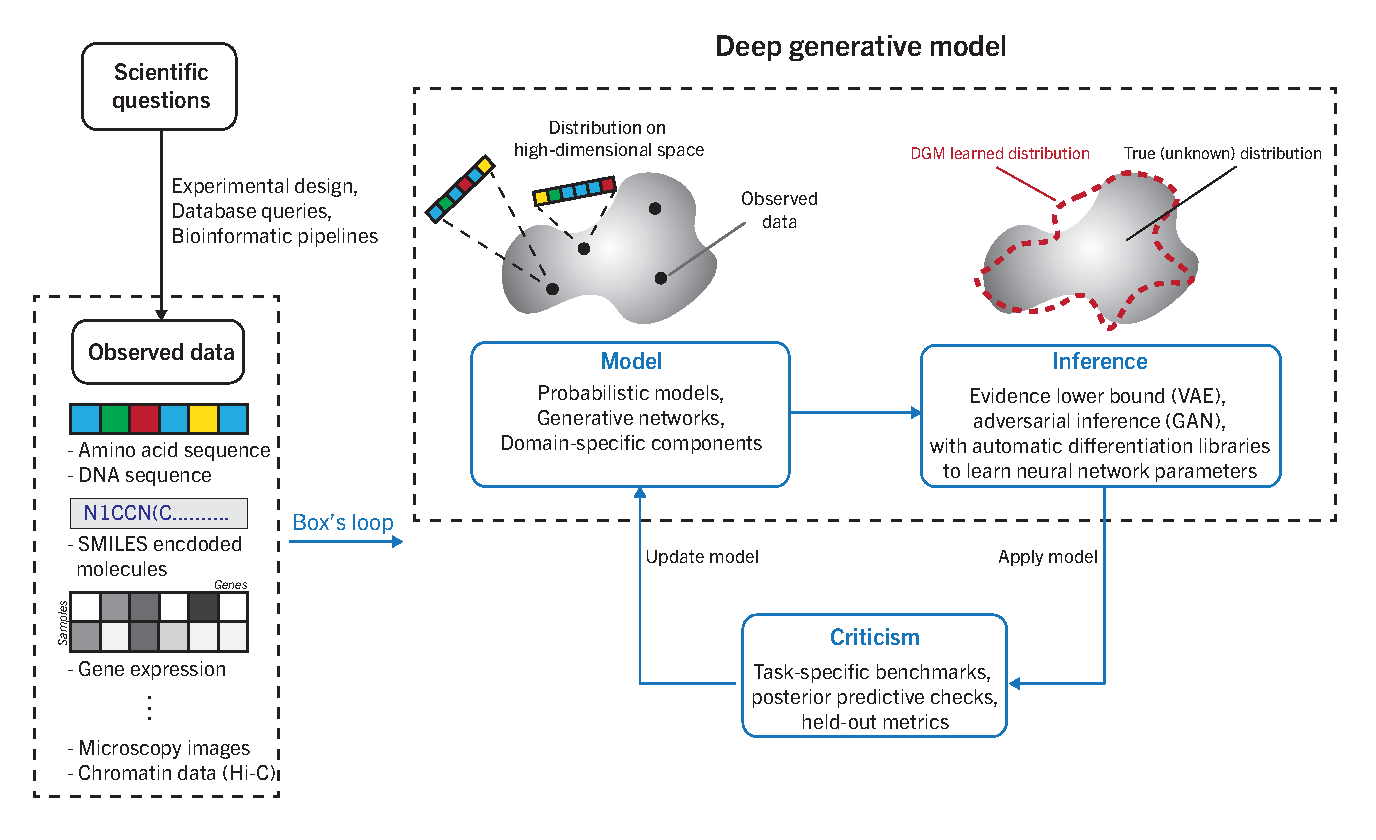
\includegraphics[width=\textwidth]{review/figures/overview_fig.pdf}
    \caption[Overview of the modeling process with DGMs.]{Overview of the modeling process with DGMs. Research in molecular biology stems from the formulation of hypotheses. Such question can be studied through the lens of a wide variety of data forms such as biological sequences, molecules, gene expression or imaging data. The broad goal of a DGM is to estimate the distribution that generated the observed data. Constructing a DGM involves iterating through the steps of Box's loop. First, a model with domain-specific components or assumptions is designed. Second, an inference procedure learns the optimal model parameters. Third, the model is criticized, which consists of benchmarking the model on datasets, or evaluating the goodness of fit of the model. Finally, the model is updated based on the criticism, starting a new iteration of the loop.}
    \label{fig:overview}
\end{figure}
